\newpage
\section{本地星系群 (Local Group)}

\subsection{本地星系群的结构}
银河系及仙女星系所在的本地星系群在天文学研究中具有特殊的地位, 无论是星系形成还是宇宙学研究, Local group都是非常重要的研究对象. 

Local group 包含约 >50个星系, 其中最大的三个成员星系为仙女星系(M31), 银河系, 三角座星系(M33, Triangulum Galaxy). 其他成员星系叫矮星系(Dwarf galaxy). 成员星系在空间并非均匀分布, 一般都聚集在这3个大星系周围. 

\subsubsection{本地星系群基本性质}

\begin{enumerate}\small 
    \item 半径$\sim 1.5$ Mpc
    \item 总质量$>2*10^{12} M_{\odot}$(主要为暗物质)
    \item 银河系-M31距离为800 Kpc,相对速度123km/s, 将在40亿年后碰撞
    \item 没有明显的物质中心, 引力势中心处在银河系和仙女星系之间
    \item 引力束缚系统
\end{enumerate}

\subsubsection{本地超星系团 Virgo Supercluster}

\begin{figure}[!htb]
    \centering
    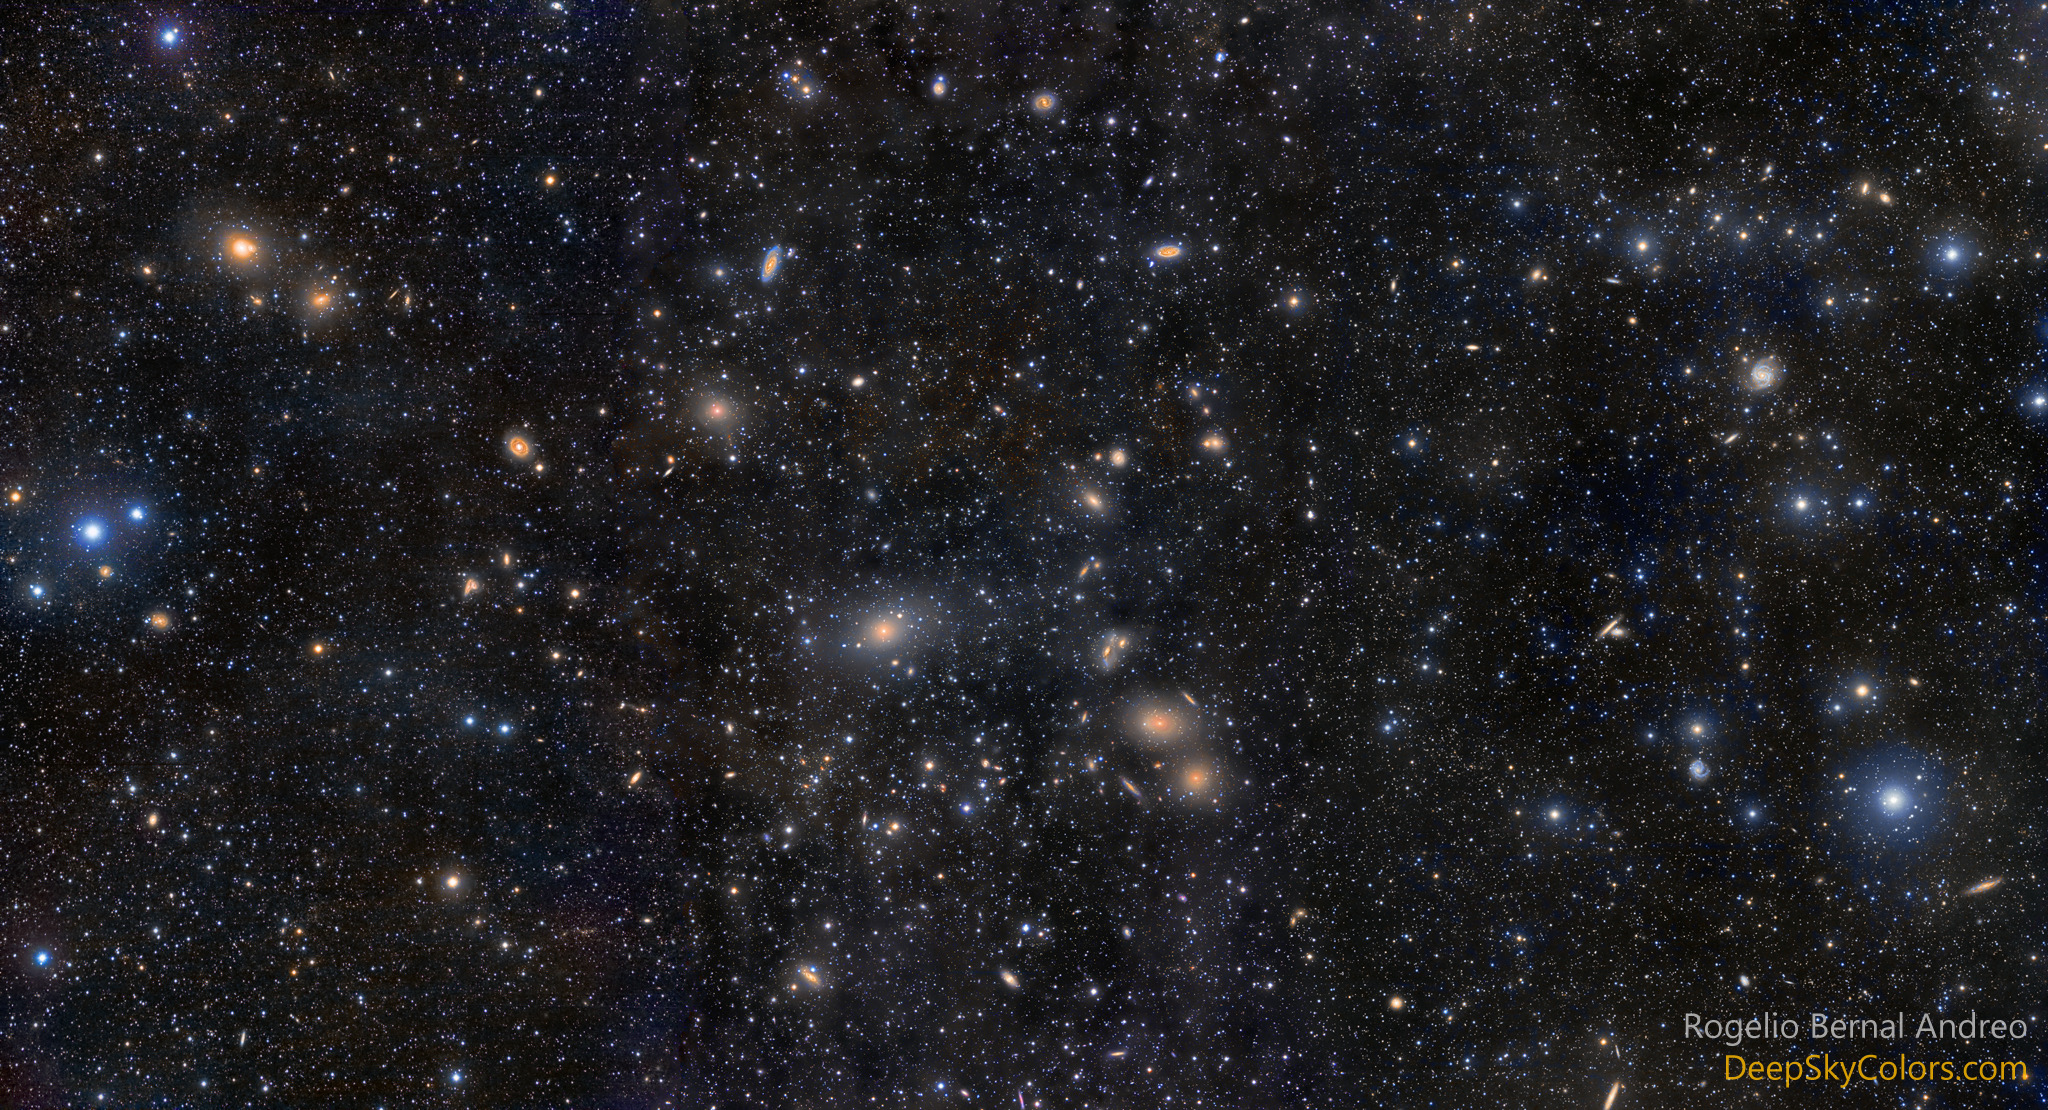
\includegraphics[width=0.42\textwidth]{GA5/室女座超星系团}
    \caption{室女座超星系团}
\end{figure}


Local group处在室女座超星系团(Virgo Spercluster)的边缘, 其中心为Virgo Cluster,它距离我们16.5 Mpc.  Virgo SC很有可能是引力束缚系统. 

Virgo SC包含约100个星系群和星系团
\begin{enumerate}\small
    \item 总质量$\sim 10^{15} M_{\odot}$
    \item 大小$\sim$33Mpc
    \item 其中心Virgo Cluster的大小为2Mpc, 在天空的面积超过1500平方度(7500个满月)
\end{enumerate}

可见宇宙中大约有1000万个类似Virgo SC

\subsubsection{超星系团 Laniakea}
夏威夷大学的Brent Tully等发现Virgo SC处在更大的所谓Laniakea超星系团中(拉尼亚凯亚). Laniakea来自夏威夷语, 表示\textbf{无尽的天堂}. 这个名称是向波利尼西亚人致敬, 彰显其利用天文知识在太平洋航行

Laniakea 主要性质:
\begin{enumerate}\small
    \item 3个超星系团: 室女座超星系团, 半人马座超星系团(其中包含 \textbf{巨引力源}), 孔雀-印第安超星系团, 长蛇座超星系团(Hydra SC)
    \item 包含约100,000星系
    \item 大小$\sim$160 Mpc, 远超过宇宙中已经位力化的平衡态的系统(星系团, 5Mpc)
    \item 其中总质量$\sim 10^{17} M_{\odot}$
    \item 本身不处于引力束缚
\end{enumerate}

\subsubsection{宇宙网络结构}
在大尺度上宇宙基本均匀、各向同性. 在$10\sim 100$Mpc的尺度上, 宇宙呈现网络状分布(Cosmic Web). 根据物质分布类型, 网络结构一般分为四种类型: 节点(Node), 墙, (Wall or sheet), 纤维结构(Filament), 空洞(Void). 

\begin{figure}[!htb]
    \centering
    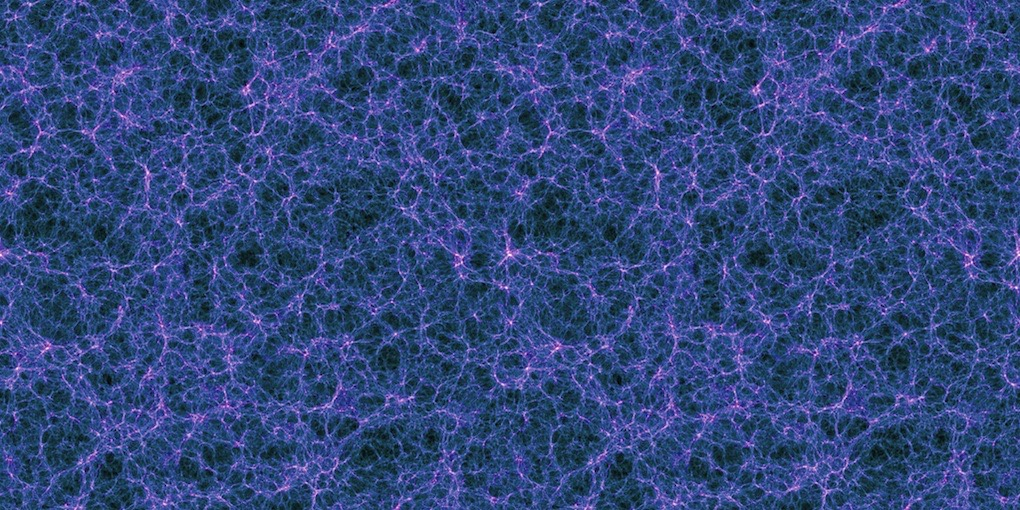
\includegraphics[width=0.42\textwidth]{GA5/宇宙物质分布的切片}
    \caption{宇宙物质分布的切片}
\end{figure}

\subsection{Local group 成员星系}

\begin{figure}[!htb]
    \centering
    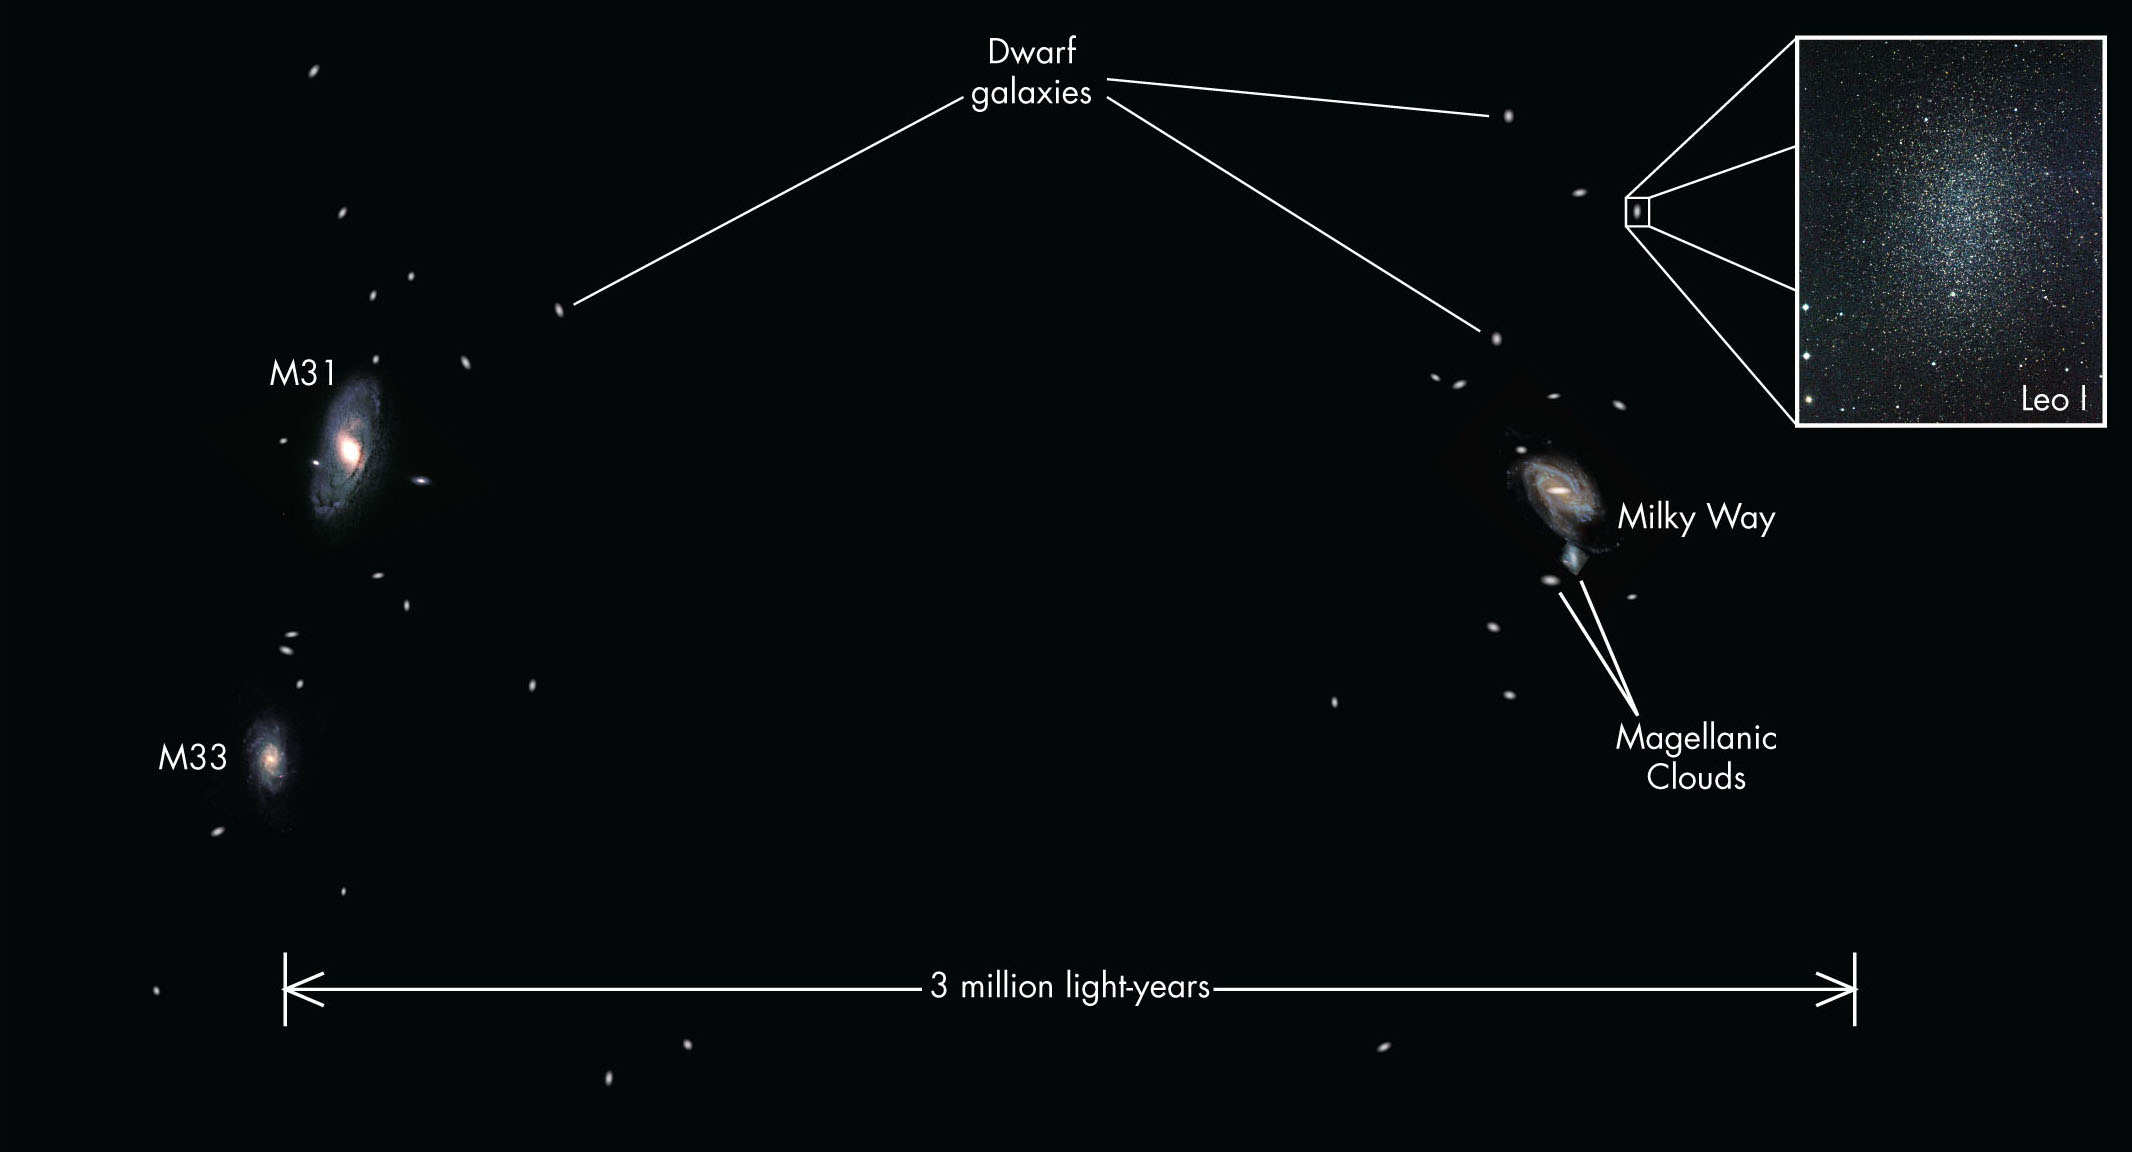
\includegraphics[width=0.42\textwidth]{GA5/Local group 成员星系}
    \caption{Local group 成员星系}
\end{figure}

寻找本地星系群的``家庭成员''天文学家的持之以恒的目标. 

\subsubsection{家长星系}
三大主要成员: 仙女星系(M31), 银河系(MW), 三角座星系(M33).
\subsubsection{仙女座星系 M31}
\begin{enumerate}\small
    \item M31, 典型的漩涡星系, 天空占据3平方度, 肉眼可见. 本星系群中的“老大”, 比银河系亮$\sim$50\%(Mv=-21.5, MW=-20.9), 尺寸大2倍. 中心核球更大
    \item 比银河系旋转更快, $\sim$260km/s, 总质量$\sim 2*10^{12}M_{\odot}$, 恒星质量$\sim 10^{11}M_{\odot}$,中性氢$\sim 5*10^9M_{\odot}$
    \item 含有$\sim$400球状星团, 比银河系多一倍
    \item 目前发现有超过30个卫星星系, 最大的为M110,M32
    \item M31中心存在一个所谓的双核, 其中一个核区中心可能是一个大质量黑洞(300万太阳质量), 周围存在一些年轻的恒星
    \item 另一个核, 可能是围绕黑洞旋转的恒星, 由于轨道椭率大, 聚集在远心点
\end{enumerate}

\begin{figure}[!htb]
    \centering
    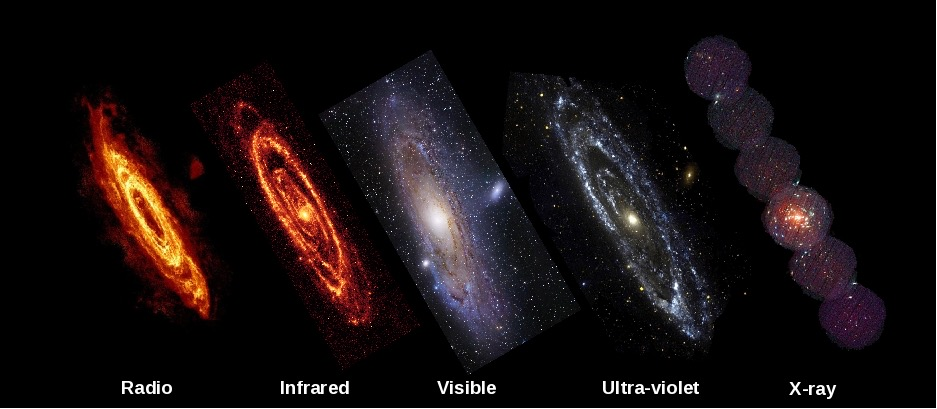
\includegraphics[width=0.42\textwidth]{GA5/M31的多波段图像}
    \caption{M31的多波段图像, 存在明显的恒星形成, 大量气体和X-ray源. }
\end{figure}

最新的观测(Van der Marel+2012)表明仙女星系相对银河系的速度为
\begin{itemize}
    \item $V_r=-109$km/s (接近银河系)
    \item $V_t = 17$km/s (切向速度)
\end{itemize}
可以从数值模拟中找到距离, 速度与Local Group接近的pair,得到LG的暗物质质量$\sim 3* 10^{12}M_{\odot}$

\subsubsection{三角座星系 M33}
Triangulum galaxy(M33)三角座星系. 距离地球273万光年, Mv=-19.5 (m=5.7),是肉眼微弱能见的最远星系. 

\begin{enumerate}\small
    \item 本地星系群的第三大成员, 漩涡星系, 距离M31为203 kpc
    \item 恒星质量$4*10^9M_{\odot}$, 气体质量$3* 10^9M_{\odot}$(主要是HI), 暗物质质量$\sim 10^{11}M_{\odot}$
    \item M33中心为一个致密星团(Nuclear star cluster), 比球状星团大, 光度$\sim 2.5*10^6L_{\odot}$, 中心无黑洞迹象(MW, M31中心都存在大质量黑洞)
    \item 可能是M31的卫星星系(束缚), 历史上曾经与M31有轨道交会/相互作用, M31-M33中间存在气体桥. 
\end{enumerate}

\begin{figure}[!htb]
    \centering
    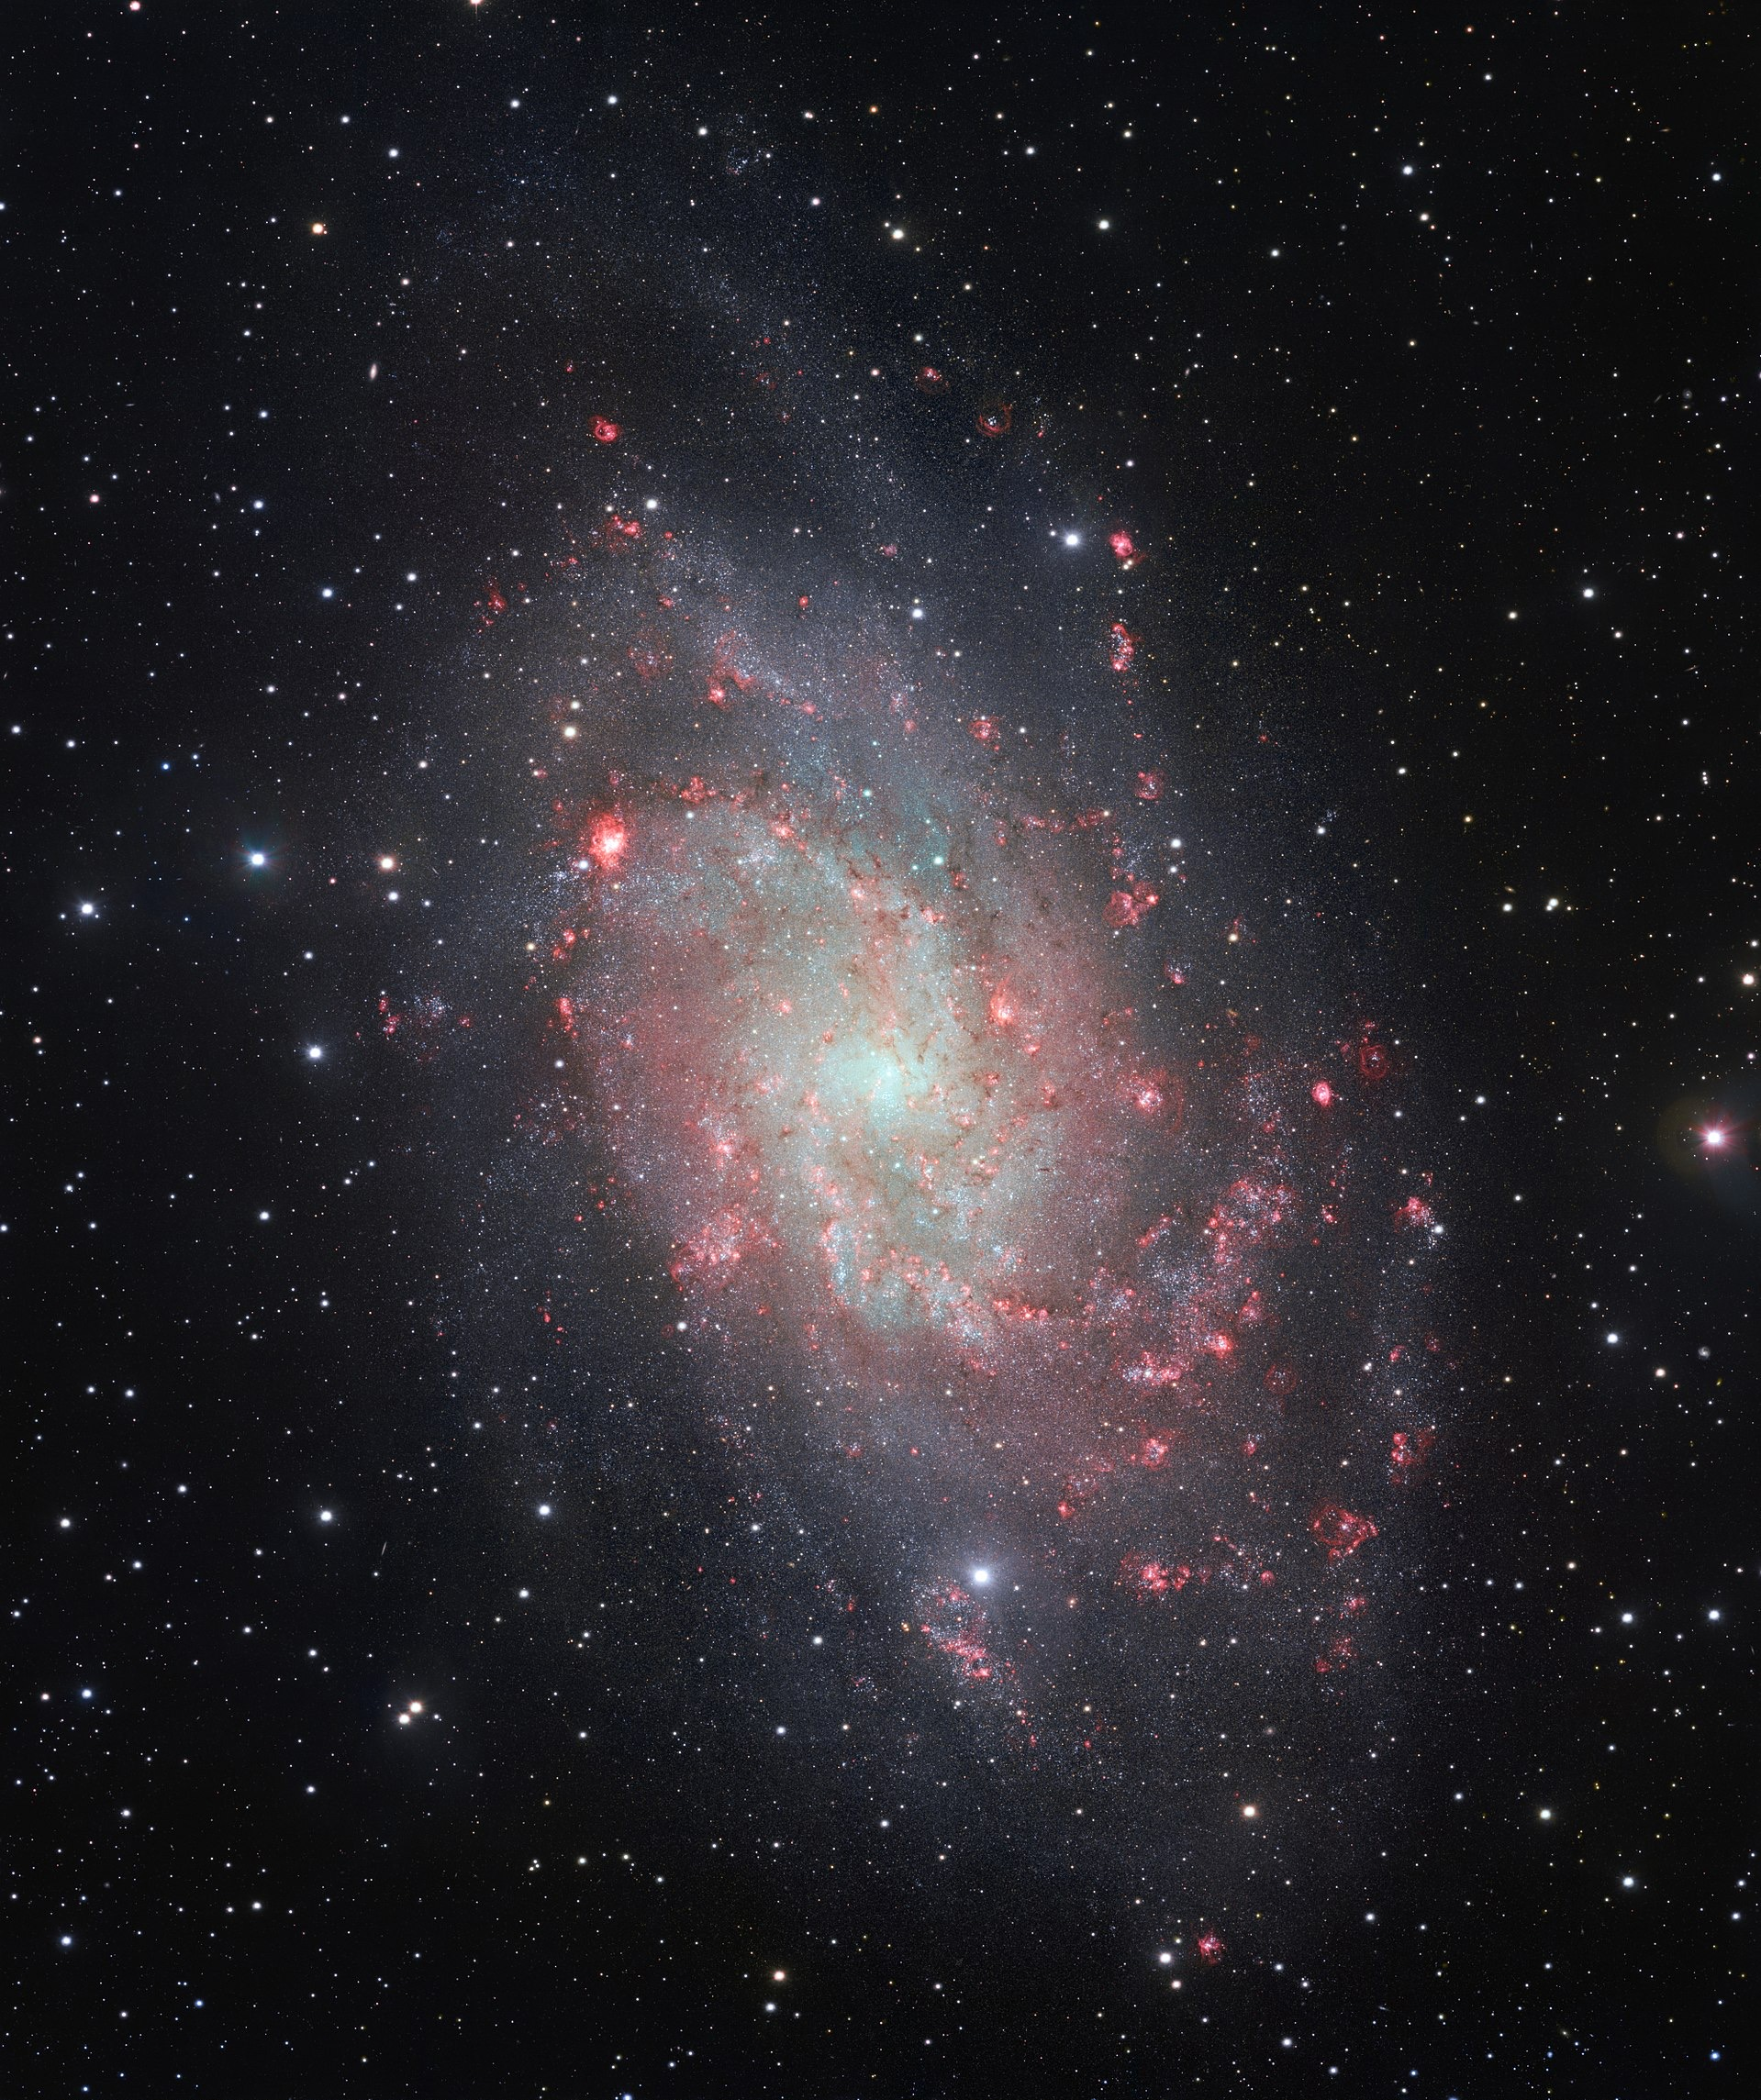
\includegraphics[width=0.12\textwidth]{GA5/M33}
    \caption{M33}
\end{figure}


\subsection{银河系卫星星系}
目前并不清楚银河系的边界有多大, 普遍认为在 200 $\sim $ 300Kpc之间. 卫星星系指距离银河系中心在此尺度范围内的矮星系. 目前观测上大约发现了银河系中有$\sim $60个卫星星系. 根据理论估计, 银河系应该有200个以上的卫星星系. 

\begin{figure}[!htb]
    \centering
    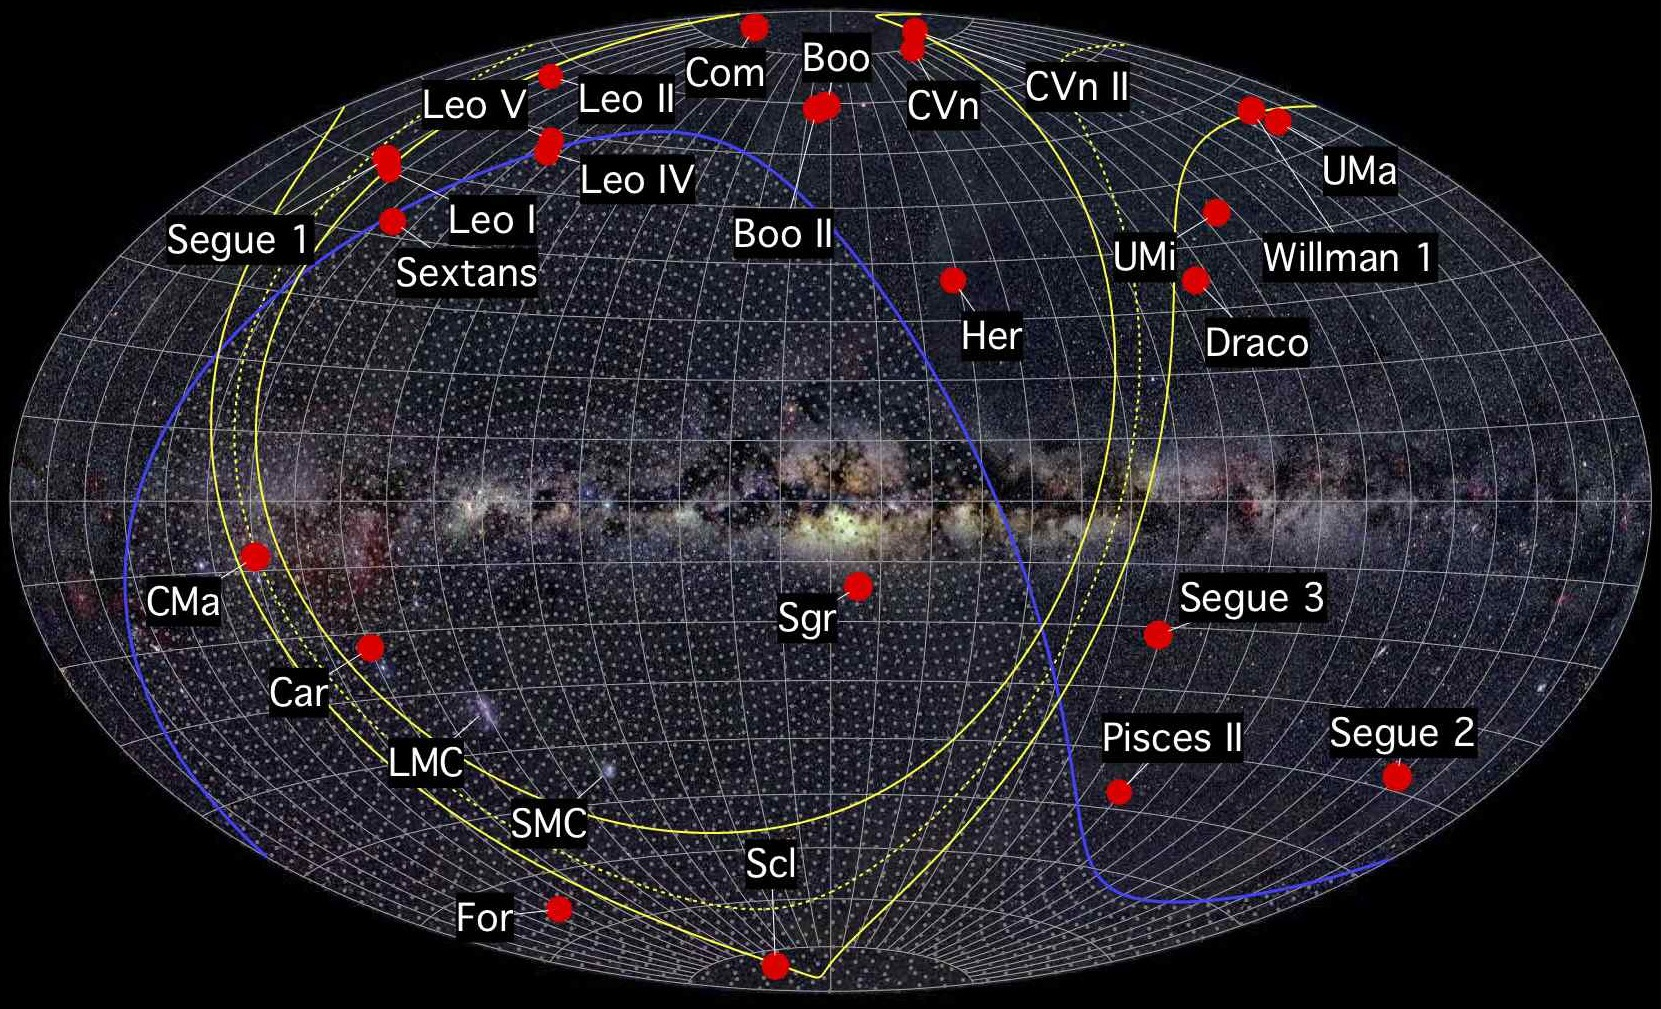
\includegraphics[width=0.309\textwidth]{GA5/卫星星系在天球上的分布}
    \caption{卫星星系在天球上的分布}
\end{figure}

\small
银河系中最著名的卫星星系是LMC(Large Magellanic Cloud, 大麦哲伦云), SMC (Small Magellanic Cloud, 小麦哲伦云). 它们分布在南半球(在北纬20度以下地区可见), 因其在天空中肉眼看上去像一团模糊的云雾状. 葡萄牙航海家麦哲伦环球航行到南半球后对其做了精确描述, 因此用其名字命名. 
\normalsize

\begin{figure}[!htb]
    \centering
    \includegraphics[width=0.309\textwidth]{GA5/LMC与SMC}
    \caption{LMC与SMC}
\end{figure}


\subsubsection{大麦哲伦云 (LMC)}
是银河系最大的卫星星系. 著名的超新星1987a来自该星系. 

\begin{figure}[!htb]
    \centering
    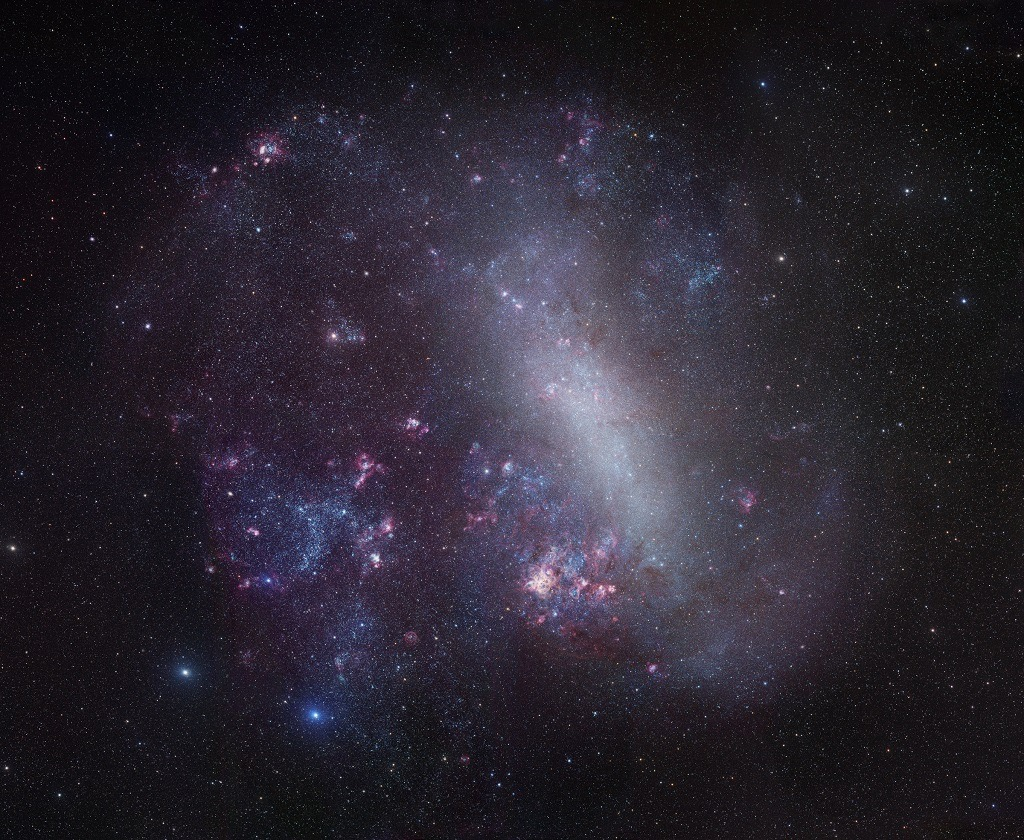
\includegraphics[width=0.309\textwidth]{GA5/大麦哲伦云}
    \caption{大麦哲伦云}
\end{figure}

\begin{enumerate}\small
    \item 尺度: 占天区$8\times 7$平方度(200满月视面积), 半径2.3Kpc, 为银河系$\sim \frac{1}{5}$
    \item 形态: 不规则星系, 具有很弱的旋臂. 可能历史上是一个漩涡星系, 潮汐作用导致其旋臂消失. 倾角$45^{\circ}$
    \item 恒星质量: $2.8*10^9M_{\odot}$ 暗物质质量$\sim 10^{10}M_{\odot}$ ,是一个暗物质占主要的星系
    \item 中性氢: LMC含有大量的恒星形成原料 (中性氢和分子氢), 质量$\sim 10 9M_{\odot}$
    \item 分子团块: 几百个,  平均$H_2$质量$\sim 10 6M_{\odot}$ 新的恒星将在这些分子团块中诞生. 
\end{enumerate}

银河系核球主序宽(恒星年龄范围跨度大)LMC主序窄, 存在大量颜色V-I$\sim$0的恒星, 具有年轻的恒星, 且金属丰度低. 

\small
大麦哲伦云是一个恒星形成星系, 被认为是``研究恒星形成的最好实验室'', 它包含约60个球状星团, 700个疏散星团, 400个行星状星云, 以及上千大质量恒星及恒星形成区. 

LMC球状星团, 有些非常古老, 跟银河系球状星团一样, 年龄超过130亿年, 有些非常年轻, 大约$\sim$350万年. 

在LMC中几乎没有年龄在130亿$\sim$4亿年之间的球状星团, 意味着其恒星形成历史非常独特. 相关研究表明(Bekki+ 2004等)表明LMC和SMC的轨道在4亿年前有一次交汇, 其强潮汐力导致了LMC随后的恒星形成(包括棒的形成)

LMC中存在大量变星. 哈佛大学天文台的Henrietta Leavitt最早于1900年左右统计了LMC中的50颗造父变星, 发现其存在周期-亮度关系. 
\normalsize

\paragraph{精确测量近邻星系/恒星距离}
对于近邻星系, 其距离测量除了三角视差, 还可以利
用两类天体用于测量距离
\begin{itemize}\small 
    \item 球状星团: 可以利用星团的颜色-星等图(CMD), 将其主序星与太阳附近主序星(颜色、绝对星等已知)比较, 移动星团CMD的纵轴使其与附近主序星重合, 从而给出距离. 
    \item 变星: 存在一类特殊的恒星, 其光度呈现周期性变化. 这种变化是由于恒星脉动引起(不稳定性). 在HR图上, 处于不稳定带内的恒星为变星. 
    \subitem 变星一般存在周期-光度关系, 其振动周期与恒星密度有关
    \begin{align*}
        T\sim \sqrt{\frac{R^3}{GM}}\sim \rho^{-0.5}
    \end{align*}
    同类型变星恒星表面温度接近, 但光度$L\sim T^4 R^2$, $R$越大, 亮度约高, 周期越长. 
\end{itemize}

\paragraph{变星(variable star)}
分为两大类: \\造父变星 (Cepheid variable) 和天琴座RR型变星, 分别以仙王座$\delta$星 (造父一) 和天琴座RR星为代表. 
\begin{itemize}\small
    \item 造父变星分为: 
    \subitem 经典造父变星, 是星族I(年轻, 富金属)恒星的变星, 质量$4\sim 20M_{\odot}$, 周期1.5-50天, 光度$\sim 10 5L_{\odot}$
    \subitem II型造父变星, 是星族II(年老, 贫金属)恒星, 质量$\sim 0.5 M_{\odot}$,  光度比同周期经典变星低1.5等
    \item 天琴座RR变星, 位于水平分支, 是核区氦燃烧的小质量恒星( $0.5 M_{\odot}$), 光度较恒定$\sim 50L_{\odot}$, 周期小于1天
\end{itemize}


\subsubsection{小麦哲伦云(SMC)}
银河系第二大卫星星系
\begin{figure}[!htb]
    \centering
    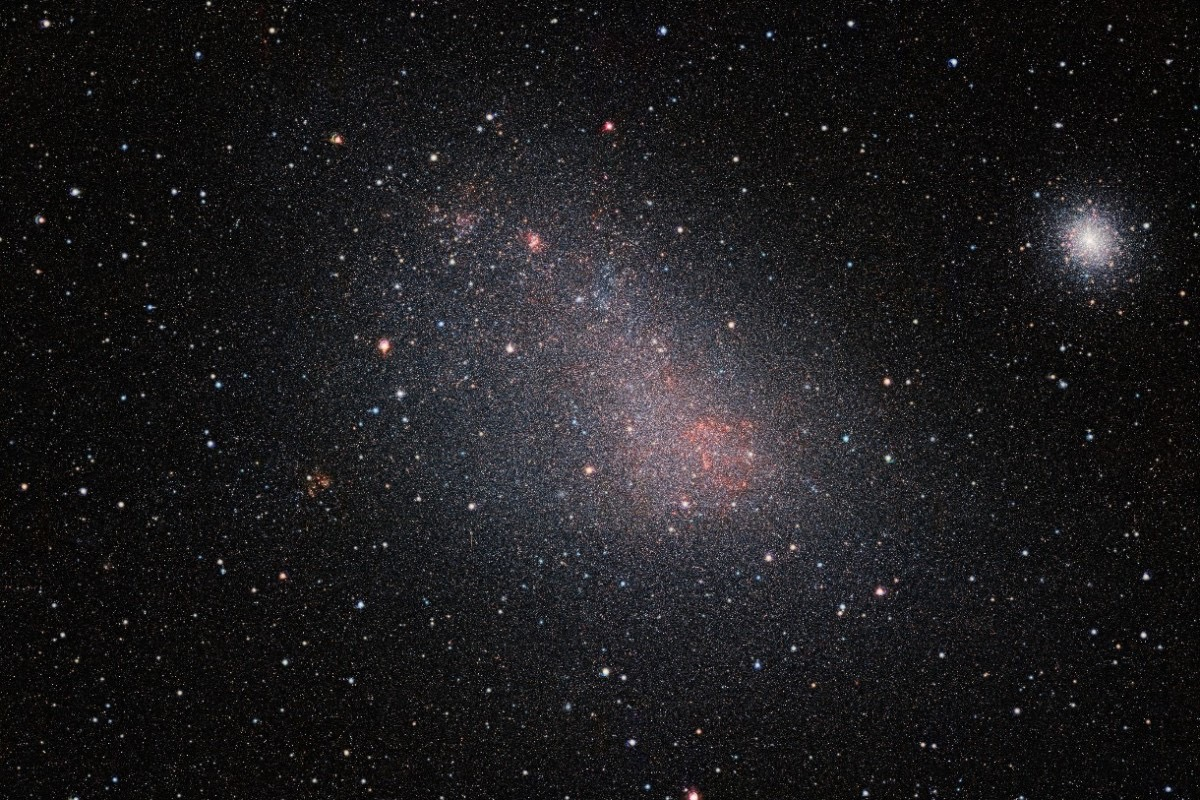
\includegraphics[width=0.309\textwidth]{GA5/小麦哲伦云}
    \caption{小麦哲伦云}
\end{figure}

\begin{enumerate}\small
    \item 尺度$\sim$ 1Kpc, 天区面积14平方度(70个满月), 距离银河系中心$\sim$ 61Kpc
    \item 恒星质量$\sim 10 8M_{\odot}$, 视星等mV=2.7,但表面亮度低, 肉眼勉强可见. 
    \item 含有大量年轻星团, 恒星金属丰度比LMC低, 但是不像LMC存在年龄间隙. 
    \item 富含中性氢, 也是恒星形成星系, 含有大量年轻星团. HI旋转曲线速度$\sim$ 60km/s. 
\end{enumerate}

\subsubsection{麦哲伦流}\small
观测表明大麦云和小麦云之间同时在银河系中运动, 但是它们之间存在明显的相互作用. 利用CO和HI观测, 发现LMC和SMC之间存在一个气体桥, 且延伸到整个天空(跨度100度, 60万光年). 其中中性氢含量约$\sim2*10^8M_{\odot}$. 

麦哲伦流中含有分子氢和中性氢, 密度非常低. 特别是对于HI,无法直接探测到其发射($\rho^2$), 一般通过背后的QSO(类星体)的吸收($\rho$)来测量其含量和速度. 通过分析麦哲伦流中气体的金属丰度, 发现它跟LMC中的气体性质接近. 

起源: 一般认为是银河系和LMC的潮汐力, 将SMC中的中性气体拉出, 形成了Magellanic Stream. 

\begin{figure}[!htb]
    \centering
    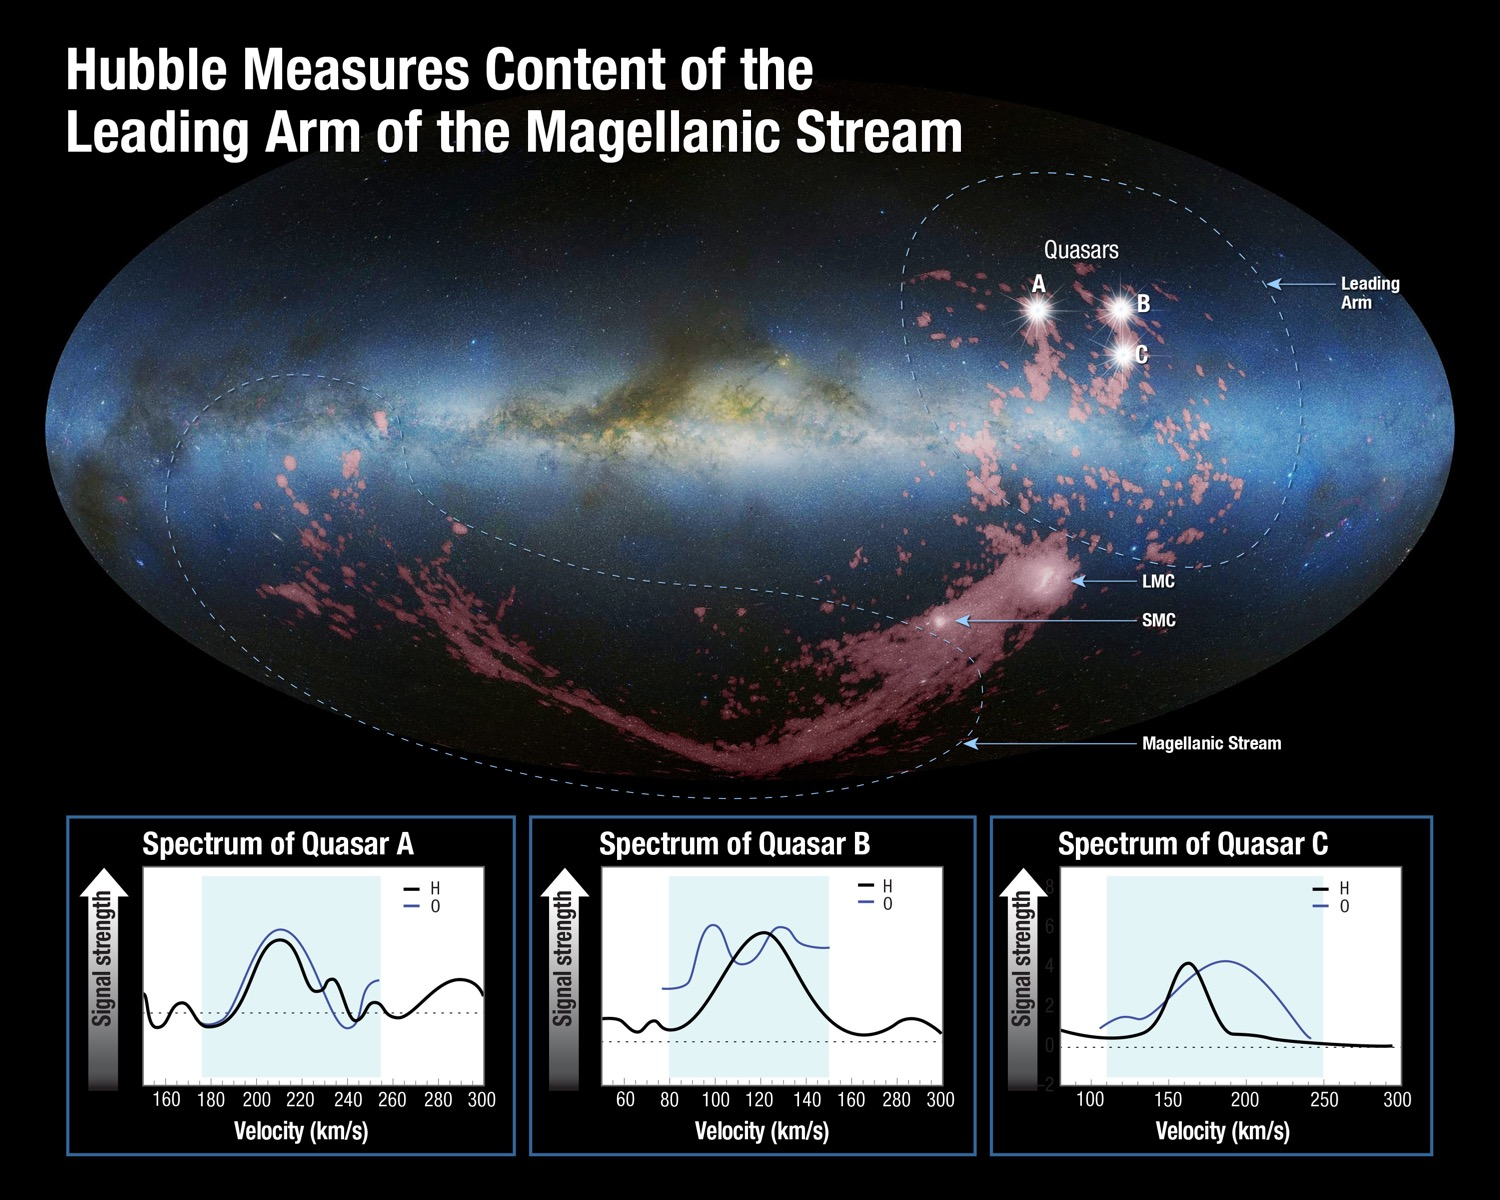
\includegraphics[width=0.309\textwidth]{GA5/麦哲伦流}
    \caption{麦哲伦流}
\end{figure}

\subsubsection{LMC 与 SMC的空间运动}

视向速度测量相对容易, 可以利用红移. 测量大/小麦哲伦云的自行非常困难. 相比恒星或者其他星系, 它们并不是点源, 在天空非常延展, 没有一个明确的中心. 同时除了整体自行以为, 它们内部的恒星也有自己的自行, 因此很难利用其中恒星来测量自行. 一般利用其整体恒星相对背景星系, 如QSO的移动, 来测量其运动. 测量耗时几年. 
\begin{itemize}
    \item LMC: 整体速度320km/s, 径向速度64km/s(离开银河系), 切向速度314km/s
    \item SMC: 整体速度217km/s, 径向速度-11km/s(接近银河系),  切向速度217km/s
\end{itemize}
\normalsize

由于LMC的速度接近逃逸速度, 普遍认为LMC/SMC并未真正被银河系束缚, 它们可能最近刚好穿越我们银河系. 

\begin{figure}[!htb]
    \centering
    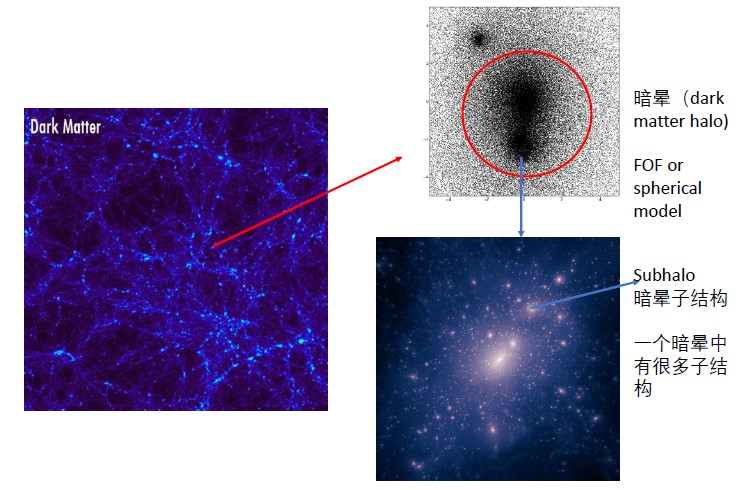
\includegraphics[width=0.42\textwidth]{GA5/物质分布与成团性}
    \caption{物质分布与成团性}
\end{figure}

\subsubsection{统计性质}

矮星系的光度甚至低于球状星团, 但是其空间分布显著大于球状星团, 处在很好的mass-size relation之上, 可以用来区分球状星团和极矮星系. 

\begin{figure}[!htb]
    \centering
    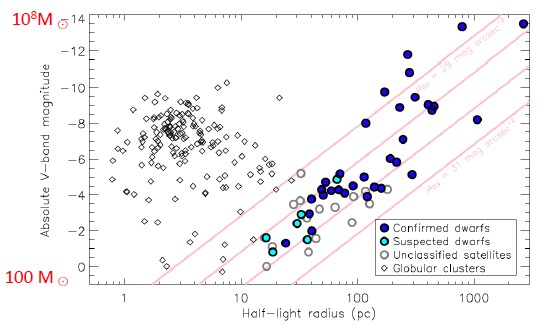
\includegraphics[width=0.42\textwidth]{GA5/光度-半光半径关系}
    \caption{光度-半光半径关系}
\end{figure}

\subsubsection{矮星系}
性质
\begin{enumerate}\small
    \item 表明亮度极低: 比LMC还低100倍以上, 非常难以探测
    \item 恒星年龄偏老: 很少有2Gyr内的年轻恒星 基本都存在天琴座RR 变星, 表明其存在年龄$>$10Gyrs的星族
    \item 金属丰度低: 大部分的金属丰度只有太阳的1\%
    \item 含有暗物质: 如果是纯恒星构成, 质量/光度$\sim 1$-$3 M_{\odot}/L_{\odot}$大部分矮星系$M/L>5$.  但具体的暗物质含量不清楚, 需要高精度光谱观测其恒星速度弥散度. 
    \item 恒星形成历史复杂: 测量矮星系的恒星形成历史非常困难, 需要分辨大量($>$200-300颗)在主序Turnoff附近的恒星. 目前基本上只有哈勃望远镜能够达到要求, 而且也只适用于较亮的矮星系 (Mv $<-3$). 
    \subitem 通过拟合其中恒星的颜色-星等图, 发现存在不同年龄的星族(3, 7, 15 Gyrs, 实际宇宙年龄$\sim $14Gyrs)
    \subitem  大部分矮星系在(z>6)之前形成了其大部分恒星. 少数矮星系有一些年轻星族, 可能因为其最近受到潮汐作用有关. 
\end{enumerate}

\begin{figure}[!htb]
    \centering
    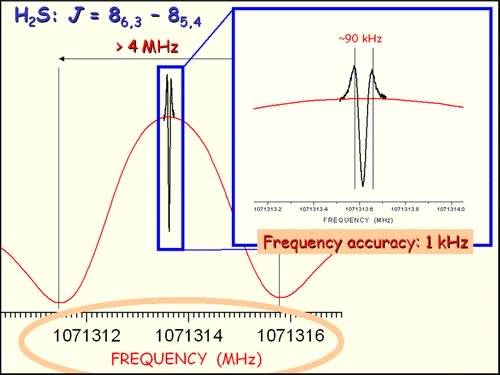
\includegraphics[width=0.309\textwidth]{GA5/谱线展宽}
    \caption{谱线展宽}
\end{figure}

\paragraph{谱线展宽}
由于光源具有一定的速度, 多普勒效应会导致单一频率的谱线偏离本征谱线. 如果速度具有一定的范围, 则导致谱线展宽. 其中心波长对应于整体运动速度导致的多普勒移动波长. 

谱线的展宽对应于速度的分布范围. 

\paragraph{矮星系的质量测量}
发光物质直接利用光度可大致得到, 一般最多存在$\sim$2-3倍的误差(来自于恒星质量/光度, $M/L$, 比对年龄和金属丰度的依赖). 总物质的含量测量非常困难. 一般是测量其中心区域的恒星视向速度弥散度$\sigma$, 再进一步利用位力定理来得到质量
\begin{align*}
    M \cong \frac{R\sigma^2}{G}
\end{align*}
$R$为矮星系的半光半径, 一般表示为$r_{1/2}$. 但位力定理的应用是基于动力学平衡的, 实际上不少矮星系处于潮汐瓦解过程中, 动力学平衡假设不一定有效. 

\paragraph{卫星星系的质量观测性质} 
\begin{itemize}\small 
    \item 大部分矮星系的速度弥散度$\sim $6km/s
    \item 总质量$\sim 10^5-10^8M_{\odot}$, 与光度有相关
    \item 质光比$\gg 2$, 意味着主要物质为暗物质, 且恒星形成效率随光度降低而降低
\end{itemize}
这些观测对星系形成物理模型和暗物质性质提出了严重挑战. 

\subsection{银河系三大著名难题}

\subsubsection{Missing satellite problem}
上世纪90年代以前数值模拟精度很低, 无法与观测进行有意义的比较. 1999年左右, 科学家完成了高精度的单个星系模拟, 发现了成百上千个“卫星星系”(其实是暗晕的子结构, 并非发光物质). 模拟的子结构(超过某个速度)$\sim$1000, 观测只有10几个. 因此有些卫星星系不见了(missing satellite). 这就是著名的Missing satellite problem. 

\paragraph{卫星星系的光度函数}
根据银河系卫星星系的绝对光度, 可以画出其光度函数. 一般越暗的卫星星系数目越多. 

\paragraph{银河系应该有多少卫星星系}
对于一个巡天, 存在巡天面积和深度. 因此, 对其观测需要修正以得到完备结果. 
\begin{enumerate}\small
    \item 巡天面积的修正. 如果某个巡天只覆盖1/5的天空, 假设分布在全天均匀, 则需要将观测数目 x5
    \item 对于给定星等Mv, 其只能在某一范围R内被探测到. 因此为了得到其在整个银河系的位力半径Rvir内的数目, 需要修正其数目为
    \begin{align*}
        N(<Rvir)=N(observed)\left( \frac{Rvir}{R} \right)^3
    \end{align*}
\end{enumerate}

\subsubsection{Too big to fall problem (大而不倒)}
观测的数据需要跟理论对比, 目前最好的理论为冷暗物质理论. 
下图为一个典型的银河系数值模拟, 中心为银河系盘. 外围是暗物质构成的暗晕, 其中包含很多暗物质组成的结构, 简称子结构(subhalo). 对于银河系, 其暗晕质量$\sim 10 ^{12}M_{\odot}$, 其中子结构可达$\sim $1000个以上, 最大子结构的质量$\sim 10 ^{11}M_{\odot}$. 

\begin{figure}[!htb]
    \centering
    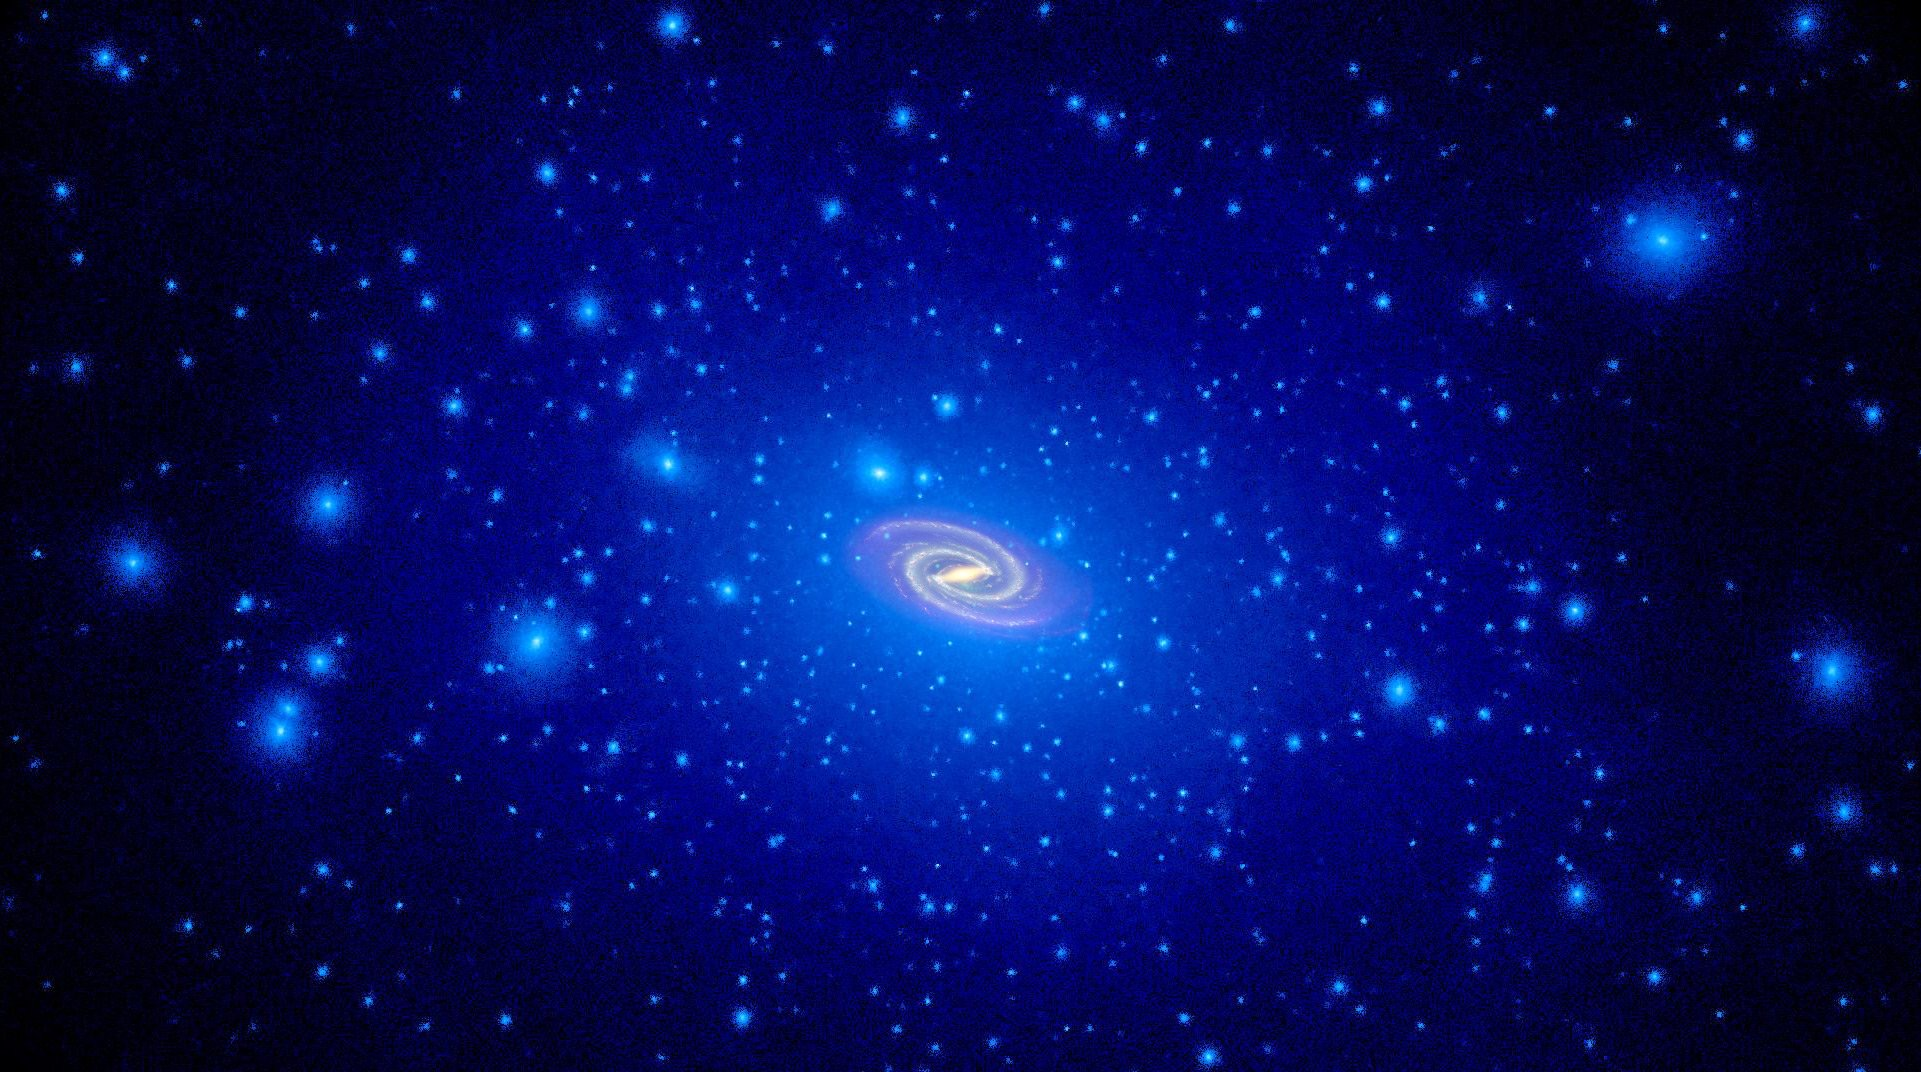
\includegraphics[width=0.479\textwidth]{GA5/银河系数值模拟}
    \caption{银河系数值模拟}
\end{figure}

一般来说, 我们认为最亮的卫星星系总是形成在最大的暗晕子结构内
因此, 可以用如下方法将观测和理论对应起来
\begin{itemize}\small
    \item 观测的卫星星系按光度排序, 选出最亮的N个卫星星系
    \item 模拟的子结构按质量或者旋转速度排序, 选出最大的N个子结构
\end{itemize}

但观测的卫星星系的旋转速度比理论预言的小. 说明观测的(亮)卫星星系不能形成于大质量子结构. 

\subsubsection{银河系卫星星系的空间分布}

下图给出银河系卫星星系相对于银河系盘的分布(图中平面为银盘). 银河系卫星星系空间分布并非球对称, 呈现两个明显特征: 
\begin{enumerate}\small
    \item 大部分聚集在盘的垂直方向上
    \item 靠近银河系中心, 密度越高
\end{enumerate}

\quad

\begin{figure}[!htb]
    \centering
    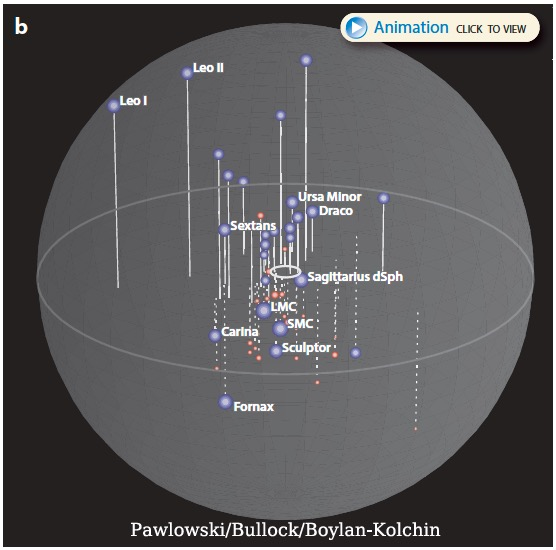
\includegraphics[width=0.309\textwidth]{GA5/银河系卫星星系的空间分布}
    \caption{银河系卫星星系的空间分布}
\end{figure}

\paragraph{卫星星系的径向分布}
径向分布可以表示为
\begin{align*}
    \rho(r)=\frac{dN(r, r+dr)}{4\pi r^2 dr}
\end{align*}
$dN$ 为某个球壳内的卫星星系数目. 

有$\sim$50\%的卫星星系分布在距离中心120Kpc以内. 越靠近中心, 卫星星系密度越高. 来自于两个效应: 
\begin{enumerate}\small
    \item 卫星星系形成时间早, 很早就掉入银河系内
    \item 动力学摩擦导致其掉向银河系中心
\end{enumerate}

\paragraph{Great Plane of MW satellites}
如果从与银河系盘平行的方向看过去(edge-on),卫星星系呈现如下图分布. 大部分卫星星系分布在与盘垂直的平面上, 分布很狭窄. 

\begin{figure}[!htb]
    \centering
    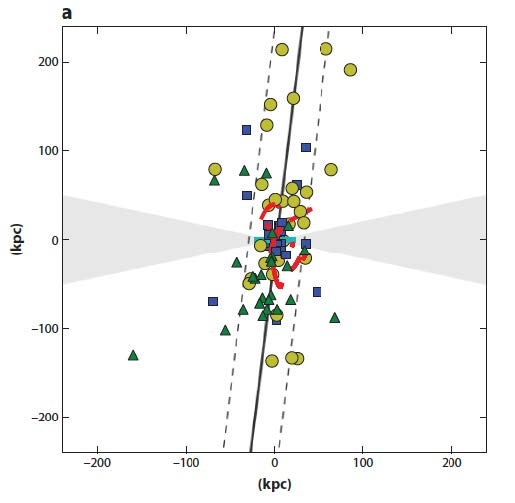
\includegraphics[width=0.309\textwidth]{GA5/银河系盘平行的方向卫星星系分布}
    \caption{银河系盘平行的方向卫星星系分布}
\end{figure}

定义卫星星系分布盘的厚度为
\begin{align*}
    \Delta=\frac{1}{R}\sqrt{\frac{\sum d_i^2}{N}}
\end{align*}
$d_i$为第$i$个卫星星系离该盘的垂直距离, $R$为卫星星系盘的最大直径, $N$为卫星星系的个数. Kroupa于2005年发现卫星星系盘的厚度$\sim$0.15, 明显大于数值模拟中卫星星系分布的厚度. 这是银河系经典的三大问题之一: satellite plane(卫星星系平面问题).

\small
随后的研究发现对于仙女星系, Centaurus A, 其卫星星系分布也存在共面的情况. 利用自行数据, Pawlowski等还发现这些卫星星系不仅共面, 而且还在该平面内运动. 理论预言中绝大多数卫星星系不存在共面现象. 意味着银河系、仙女星系中卫星星系平面有着其特殊的物理起源. 
\normalsize